
\section*{Koloniepikker}
\flushright

\includegraphics[width=4em]{logo-new.png}

\includegraphics[width=4em]{logo-new.png}

\includegraphics[width=4em]{logo-new.png}
\flushleft

Een koloniepikker is een instrument waarmee microbi\"ele kolonies die op een
vaste voedingsbodem groeien automatisch kunnen worden gelocaliseerd, opgepikt
en gedupliceerd op een vaste of vloeibare voedingsbodem. Doorgaans wordt een
petrischaal aangebracht op de lichtplaat van de koloniepikker, waarna
algoritmen voor beeldanalyse de juiste kolonies uitkiezen en een robotarm
aansturen om die kolonies te bemonsteren. Dergelijke toestellen worden zowel in
onderzoekslaboratoria als in industri\"ele omgevingen gebruikt, bijvoorbeeld om
voedings- of bloedstalen te analyseren.

De beeldverwerkingssoftware krijgt de foto van een petriplaat te zien onder de
vorm van een bitmap. Dit is niets anders dan een rechthoekig rooster waarvan de
vakjes bits genoemd worden omdat ze slechts twee toestanden kunnen aannemen.
Elke bit van het rooster is ofwel leeg (voorgesteld door een spatie) of wordt
bedekt door een kolonie (voorgesteld door een hekje: \#). Als voorbeeld zie je
hieronder een bitmap waarop een aantal kolonies te zien zijn. In een bitmap
wordt een kolonie gevormd door een gebied van aangrenzende bedekte bits. Bits
worden hierbij aangrenzend genoemd als ze een gemeenschappelijke zijde hebben.
De software zal een gebied van aangrenzende bedekte bits echter nooit als een
kolonie beschouwen, als het bits op de buitenste rand van de bitmap bevat.

\begin{figure}[H]
  \begin{center}
    \centerline{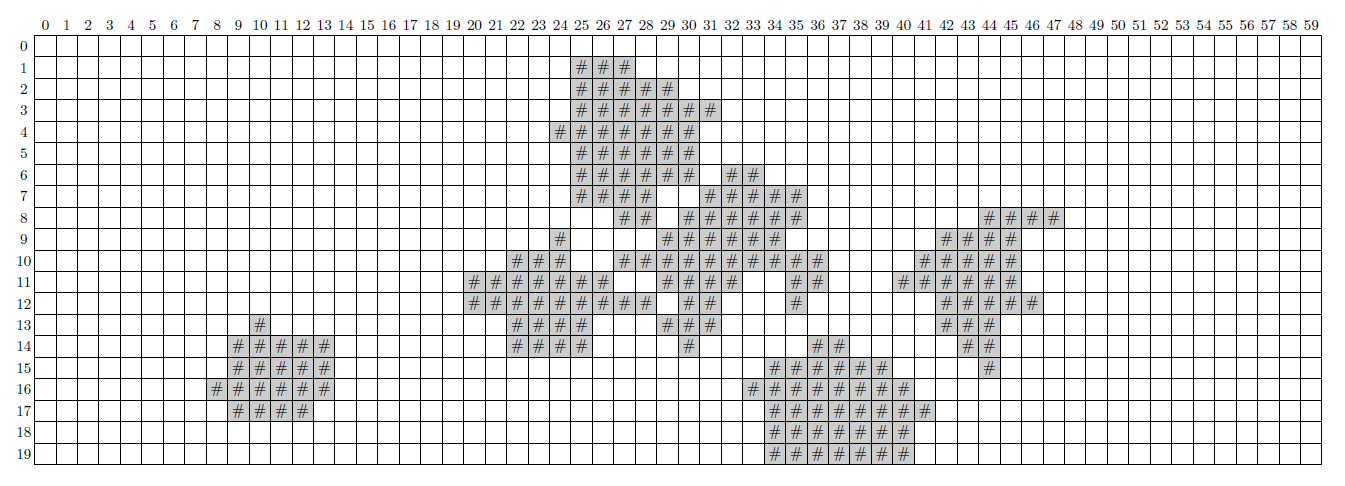
\includegraphics[scale=0.30]{koloniepikker/colony_bitmap.png}}
    \caption{Bitmap gemaakt van een petriplaat. Deze bitmap is een rechthoekig
        rooster met 20 rijen en 60 kolommen, waarbij de bits die bedekt zijn
        door bacteri\"ele kolonies worden aangeduid door hekjes (\#). Deze
        bitmap telt zes gebieden van aangrenzende bezette bits, maar slechts
        vijf daarvan worden als kolonies beschouwd, omdat er \'e\'en gebied bits
        heeft die op de buitenste rand van de bitmap liggen.}
  \end{center}
\end{figure}

\subsection*{Input}

De input bestaat zoals gebruikelijk eerst een lijn die het aantal gevallen
aanduid, gevolgd door de verschillende gevallen. Per geval krijgen we eerst een
lijn die dit geval beschrijft. Deze bevat 3 gehele getallen, gescheiden door
spaties. Het eerste en tweede getal zijn de hoogte en breedte van de
matrixvoorstelling van de petrischaal. Het derde is de minimum-grootte voor een
aaneensluiting van \#'s om mee te tellen als kolonie. Vlekken met een grootte
kleiner dan dit minimum worden als ruis beschouwd en verwaarloosd.

Hierop volgt dan het gespecifieerde aantal lijnen van gegeven breedte. Deze zijn
gevuld met spaties en \#'s.

\subsubsection*{Voorbeeldinput}

\begin{verbatim}
2
20 61 1

                         ###
                         #####
                         #######
                        #######
                         ######
                         ###### ##
                         ####  #####
                           ## ######        ####
                        #    ######       ####
                      ###  ##########    #####
                    #######  ####  ##   ######
                    ######### ##   #      #####
          #           ####   ###          ###
         #####        ####    #     ##     ##
         #####                    ######    #
        ######                   ########
         ####                     ########
                                  #######
                                  #######
4 8 1

 # ## ##
 # ## ##

\end{verbatim}

\subsection*{Output}

Per geval verwachten we enerzijds een geheel getal dat het aantal kolonies
voorsteld, en anderszijds de gemiddelde grootte van de kolonies. Vergeet geen
rekening te houden met de minimum-grootte. Deze twee getallen verwachten we op
een enkele lijn, gescheiden door een spatie. De gemiddelde grootte zal een
kommagetal zijn, afgerond op 3 cijfers na de komma.

\subsubsection*{Voorbeeldoutput}

\begin{verbatim}
5 32.2
3 3.333
\end{verbatim}
